\providecommand{\main}{..}		% Override relative path to the main file (already set in main file)
\documentclass[../InterneDSLs.tex]{subfiles}
\begin{document}

\chapter{Bau des Prototypen}

\section{Aufbau}
Die Verarbeitung der Grammatik erfolgt nach dem folgenden Schema:
\begin{itemize}
	\item Parsen der Grammatik
	\item Aufbau des Syntax-Baumes (aus Java-Typen)
	\item Abbildung in einen Graphen, der die Aufrufreihenfolge abbildet
	\item Generierung der Interfaces
\end{itemize}

\section{Parser}
Als Parser-Generator wurde ANTLR4 verwendet, der Parser zu einer EBNF-Grammatik in Java generieren kann. Dafür verwendet ANTLR aber eine unübliche Syntax, die sich an einer alten EBNF-Variante orientiert.

Der von ANTLR generierte Parser wird von einem Listener erweitert, der aus den EBNF-Konstrukten (die praktisch Strings entprechen) einen Baum aus eigenen Klassen generiert. Dadurch wird eine Typ-Sicherheit hergestellt, die durch die EBNF selbst nicht gegeben ist.

\section{Abbildung von EBNF auf Interfaces}
Zuerst wird die in EBNF geschriebene Grammatik in einen Baum aus Java-Objekten transformiert. Dadurch wird eine Typ-Sicherheit hergestellt und Methoden implementiert werden, die das Traversieren des Baumes vereinfachen. Abbildung~\ref{FIG:TypesBNF} zeigt die Typen und ihre Beziehungen untereinander. Diese Typen finden sich auch in den Regeln der EBNF-Grammatik (Abbildung~\ref{FIG:EBNFGrammar}) wieder.

Um die Interfaces generieren zu können, müssen die Kanten der Graphen zwischen den Scopes, auf Interfaces abgebildet werden.

\begin{figure}[ht]
\centering
\includegraphics[width=\linewidth]{\main/10_Pictures/BNF-Types}
\caption{Typen des BNF-Baumes}
\label{FIG:TypesBNF}
\end{figure}

\begin{figure}[ht]
\lstinputlisting[linerange={3-28,38-45},caption={EBNF-Grammatik (Auszug)\label{FIG:EBNFGrammar}}]{Bnf.g4}
\end{figure}

\subsection{Kante mit einem Knoten}
Im einfachsten Fall von einer Kante, die nur einen Sequenz-Knoten beinhaltet, kann man den ein Interface mit dem Namen des Knotens und dem nächsten Scope als Rückgabewert erstellen. Grafik~\ref{FIG:OneElementNode} zeigt, wie eine Abbildung aussehen kann.
\begin{figure}[ht]
\centering
  \begin{subfigure}[c]{0.49\textwidth}
    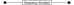
\includegraphics[width=.95\linewidth]{\main/10_Pictures/Nodes_one-element}
    \caption{Diagramm eines Sequenz-Knotens}
    \label{FIG:DiagramOneElementNode}
  \end{subfigure}
  \begin{subfigure}[c]{0.49\textwidth}
    \lstinputlisting[language=Java,caption={Java-Interface aus einem Sequenz-Knoten\label{FIG:JInterfaceOneElementNode}}]{Scope_one-element.java}
  \end{subfigure}
  \caption{Diagramm und Interface eines Sequenz-Knotens}
  \label{FIG:OneElementNode}
\end{figure}

Falls man einen Knoten überspringen kann (bzw. optional ist), muss man vom folgenden Scope (Listing~\ref{FIG:JInterfaceOptionalNode}) erben, um dessen Methoden aufrufen zu können und damit die eigene(n) auslassen zu können.
\begin{figure}[ht]
\centering
  \begin{subfigure}[c]{0.49\textwidth}
    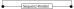
\includegraphics[width=.95\linewidth]{\main/10_Pictures/Nodes_optional}
    \caption{Diagramm eines optionalen Sequenz-Knotens}
    \label{FIG:DiagramOptionalNode}
  \end{subfigure}
  \begin{subfigure}[c]{0.49\textwidth}
    \lstinputlisting[language=Java,caption={Java-Interface aus einem optionalen Sequenz-Knoten\label{FIG:JInterfaceOptionalNode}}]{Scope_optional.java}
  \end{subfigure}
  \caption{Diagramm und Interface eines optionalen Sequenz-Knotens}
  \label{FIG:OptionalNode}
\end{figure}

\subsection{Kante mit Alternativen}
Falls eine Kante mehrere Alternativen enthält, können die alternativen je als eine Methode in einem Interface implementiert werden, die jeweils den folgenden Scope zurück geben (siehe Abbildung~\ref{FIG:AlternativeNode}).
\begin{figure}[ht]
\centering
  \begin{subfigure}[c]{0.49\textwidth}
    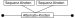
\includegraphics[width=.95\linewidth]{\main/10_Pictures/Nodes_alternative}
    \caption{Diagramm alternativer Knoten}
    \label{FIG:DiagramAlternativeNode}
  \end{subfigure}
  \begin{subfigure}[c]{0.49\textwidth}
    \lstinputlisting[language=Java,caption={Java-Interface aus alternativen Knoten\label{FIG:JInterfaceAlternativeNode}}]{Scope_alternative.java}
  \end{subfigure}
  \caption{Diagramm und Interface alternativer Knotens}
  \label{FIG:AlternativeNode}
\end{figure}

\subsection{Kante mit Schleife}
Eine Wiederholung wird mit einem Schleifen-Knoten modelliert, der einen Sequenz-Knoten beinhaltet. Für eine Wiederholung, die kein Vorkommen erlaubt, reicht ein Scope, der vom Folge-Scope erbt; damit kann der Methodenaufruf vom Schleifen-Scope übersprungen werden.

Falls die Wiederholung mindestens ein Vorkommen voraussetzt muss ein zusätzlichen Interface eingeführt werden, das dieselbe Methode deklariert und nicht vom Folge-Interface erbt, um einen Methodenaufruf zu erzwingen (Listing~\ref{FIG:JInterfaceLoopNode}).
\begin{figure}[ht]
\centering
  \begin{subfigure}[c]{0.49\textwidth}
    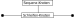
\includegraphics[width=.95\linewidth]{\main/10_Pictures/Nodes_loop}
    \caption{Diagramm eines Schleifen-Knotens}
    \label{FIG:DiagramLoopNode}
  \end{subfigure}
  \begin{subfigure}[c]{0.49\textwidth}
    \lstinputlisting[language=Java,caption={Java-Interface aus einem Schleifen-Knoten\label{FIG:JInterfaceLoopNode}}]{Scope_loop.java}
  \end{subfigure}
  \caption{Diagramm und Interface eines Schleifen-Knotens}
  \label{FIG:LoopNode}
\end{figure}

\subsection{Sequenz von Knoten}
Tritt eine Sequenz von Knoten auf, muss für jeden Knoten ein Interface mit einer Methode generiert werden, um die Aufruf-Reihenfolge zu gewährleisten. Abbildung~\ref{FIG:SequenceNode} zeigt ein Beispiel mit zwei Knoten in einer Sequenz.
\begin{figure}[ht]
\centering
  \begin{subfigure}[c]{0.49\textwidth}
    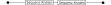
\includegraphics[width=.95\linewidth]{\main/10_Pictures/Nodes_sequence}
    \caption{Diagramm einer Sequenz von Knoten}
    \label{FIG:DiagramSequenceNode}
  \end{subfigure}
  \begin{subfigure}[c]{0.49\textwidth}
    \lstinputlisting[language=Java,caption={Java-Interfaces aus einer Sequenz von Knoten\label{FIG:JInterfaceSequenceNode}}]{Scope_sequence.java}
  \end{subfigure}
  \caption{Diagramm und Interface einer Sequenz von Knotens}
  \label{FIG:SequenceNode}
\end{figure}


\section{Schwierigkeiten beim Bau}
Beim Erstellen des Prototypen traten einige Schwierigkeiten auf. Die größten werden in diesem Abschnitt besprochen: die Behandlung der Rekursion der EBNF-Grammatik und die der Typen.

\subsection{Behandlung der Rekursion}

\subsection{Typen}

\subsubsection{Mapping auf Typen der Hostsprache}
- NTs -> Methoden (Einschränungen)

- Interfacenamen beliebig

\subsubsection{Generierung von Typen aus EBNF-Regeln}


\section{Einschränkungen bei der Grammatik}
Die EBNF-Grammatik kann nicht beliebig formuliert sein.

\subsection{Startregel}
In der Grammatik muss eine Startregel definiert sein, die nur ein Nicht-Terminal beinhaltet. Daraus wird das erste Interface als Einstiegspunkt generiert.

\subsection{Lexer-Regeln}
Für jede Lexer-Regel sollte es eine entsprechende Parser-Regel geben, die nur die jeweilige Lexer-Regel beinhaltet. Dadurch kann der Listener des Parsers die Typen auch verarbeiten.

Falls eine Regel innerhalb einer anderen vorkommt, ohne ein Trennsymbol zu einer anderen, darf es ebenfalls keine Lexer-Regel sein, um vom Listener erkannt zu werden.


\chapter{Testlauf mit anschaulichem Beispiel}


\section{Optimierungspotenzial}


\section{Varianten}


\end{document}
